%\documentclass[a4paper,10pt]{article}
\documentclass{iiufrgs}
\usepackage[utf8]{inputenc}
\usepackage{enumitem}
\usepackage{url}
\usepackage{setspace}
\usepackage[list-style=extra-tabular]{acro}
\usepackage{graphicx}
%\usepackage[brazilian]{babel}
  
\setdescription{topsep=1em,parsep=0pt,partopsep=0pt,itemsep=0pt}
\setitemize{topsep=1em,parsep=0pt,partopsep=0pt,itemsep=0pt}
\setenumerate{topsep=1em,parsep=0pt,partopsep=0pt,itemsep=0pt}

%capa
\course{\cgcc}
\title{Implementação de alta disponibilidade em uma empresa prestadora de serviços para Internet}
\author{Emer}{Bruno}
\advisor[]{Martinotto}{André Luis}
\location{Caxias do Sul}{}
\bibpunct{(}{)}{;}{a}{,}{,}

%declaracoes siglas
\DeclareAcronym{TI}{
  short = TI,
  long  = Tecnologia da Informação,
  class = abbrev
}
\DeclareAcronym{ECC}{
  short = ECC,
  long  = \textit{Error correction code},
  class = abbrev
}
\DeclareAcronym{RAID}{
  short = RAID,
  long  = \textit{Redundant array of independent disks},
  class = abbrev
}
\DeclareAcronym{SPOF}{
  short = SPOF,
  long  = \textit{Single point of failure},
  class = abbrev
}
\DeclareAcronym{MTBF}{
  short = MTBF,
  long  = \textit{Mean time between failures},
  class = abbrev
}
\DeclareAcronym{MTTR}{
  short = MTTR,
  long  = \textit{Mean time to repair},
  class = abbrev
}
\DeclareAcronym{SLA}{
  short = SLA,
  long  = \textit{Service level agreement},
  class = abbrev
}
\DeclareAcronym{VM}{
  short = VM,
  long  = \textit{Virtual machine},
  class = abbrev
}
\DeclareAcronym{OS}{
  short = OS,
  long  = \textit{Operating system},
  class = abbrev
}
\DeclareAcronym{PC}{
  short = PC,
  long  = \textit{Personal computer},
  class = abbrev
}
\DeclareAcronym{JVM}{
  short = JVM,
  long  = \textit{Java virtual machine},
  class = abbrev
}
\DeclareAcronym{VMM}{
  short = VMM,
  long  = \textit{Virtual machine monitor},
  class = abbrev
}
\DeclareAcronym{ISA}{
  short = ISA,
  long  = \textit{Instruction set architecture},
  class = abbrev
}
\DeclareAcronym{IVT}{
  short = IVT,
  long  = \textit{Intel virtualization technology},
  class = abbrev
}
\DeclareAcronym{AMD-V}{
  short = AMD-V,
  long  = \textit{AMD virtualization},
  class = abbrev
}
\DeclareAcronym{KVM}{
  short = KVM,
  long  = \textit{Kernel-based virtual machine},
  class = abbrev
}
\DeclareAcronym{JIT}{
  short = JIT,
  long  = \textit{Just-in-time},
  class = abbrev
}
\DeclareAcronym{DNS}{
  short = DNS,
  long  = \textit{Domain name system},
  class = abbrev
}
\DeclareAcronym{NAT}{
  short = NAT,
  long  = \textit{Network address translation},
  class = abbrev
}
\DeclareAcronym{IPv6}{
  short = IPv6,
  long  = \textit{Internet protocol version 6},
  class = abbrev
}
\DeclareAcronym{WHM}{
  short = WHM,
  long  = \textit{WebHost manager},
  class = abbrev
}
\DeclareAcronym{PRTG}{
  short = PRTG,
  long  = \textit{Paessler router traffic grapher},
  class = abbrev
}
\DeclareAcronym{ADSL}{
  short = ADSL,
  long  = \textit{Asymmetric Digital Subscriber Line},
  class = abbrev
}
\DeclareAcronym{PPPoE}{
  short = PPPoE,
  long  = \textit{Point-to-point protocol over ethernet},
  class = abbrev
}
\DeclareAcronym{API}{
  short = API,
  long  = \textit{Application programming interface},
  class = abbrev
}
\DeclareAcronym{LTS}{
  short = LTS,
  long  = \textit{Long term support},
  class = abbrev
}
\DeclareAcronym{FTP}{
  short = FTP,
  long  = \textit{File transfer protocol},
  class = abbrev
}
\DeclareAcronym{NRPE}{
  short = NRPE,
  long  = \textit{Nagios remote plugin executor},
  class = abbrev
}
\DeclareAcronym{SVN}{
  short = SVN,
  long  = \textit{Subversion},
  class = abbrev
}
\DeclareAcronym{PHP}{
  short = PHP,
  long  = \textit{Personal home page},
  class = abbrev
}
\DeclareAcronym{ASP}{
  short = ASP,
  long  = \textit{Active server pages},
  class = abbrev
}
\DeclareAcronym{SMTP}{
  short = SMTP,
  long  = \textit{Simple mail transfer protocol},
  class = abbrev
}
\DeclareAcronym{POP}{
  short = POP,
  long  = \textit{Post office protocol},
  class = abbrev
}
\DeclareAcronym{IMAP}{
  short = IMAP,
  long  = \textit{Internet message access protocol},
  class = abbrev
}
\DeclareAcronym{XMPP}{
  short = XMPP,
  long  = \textit{Extensible messaging and presence protocol},
  class = abbrev
}
\DeclareAcronym{SSH}{
  short = SSH,
  long  = \textit{Secure shell},
  class = abbrev
}
\DeclareAcronym{IP}{
  short = IP,
  long  = \textit{Internet protocol},
  class = abbrev
}



\begin{document}

\maketitle

\begin{titlepage}
%\setcounter{page}{2} - Inclui o número da página
%\thispagestyle{headings}
\vfill

\begin{center}
{\setlength{\unitlength}{1cm}\makebox(12,6.5){\parbox[c]{12cm}{\setlength{\parskip}{0.8cm}\center\vskip -1.2cm\LARGE{\bf Implementação de alta disponibilidade em uma empresa prestadora de serviços para Internet}\par \normalsize por\par \large Bruno Emer\par}}}
\end{center}

{\large Projeto de Diplomação submetido ao curso de Bacharelado em Ciência da Computação do Centro de Ciências Exatas e da Tecnologia da Universidade de Caxias do Sul, como requisito obrigatório para graduação.}

\vfill

\begin{center}
{\Large\bf Projeto de Diplomação}
\end{center}

\vfill

\begin{singlespace}
Orientador: {André Luis Martinotto\par}

Banca examinadora:\par
\hspace{1cm} {\setlength{\unitlength}{1cm}
\makebox(9,1){\parbox[c]{9cm}{\center Maria de Fatima Webber do Prado Lima\\ CCTI/UCS}}}\par
\hspace{1cm} {\setlength{\unitlength}{1cm}
\makebox(9,1){\parbox[c]{9cm}{\center Ricardo Vargas Dorneles\\ CCTI/UCS}}}\par

\vfill

\hfill{\setlength{\unitlength}{1cm}\makebox(9,2.5){\parbox[c]{9cm}{\setlength{\parskip}{0.8cm}\center\vskip -1.2cm Projeto de Diplomação apresentado em\\ x de julho de 2016\par Daniel Luís Notari\\ Coordenador}}}

\end{singlespace}

\end{titlepage}


\tableofcontents

\chapter*{Lista de siglas}
\printacronyms[include-classes=abbrev,name=]
%\chapter*{Lista de acrônimos}
%\begin{acronym}[XXXXXXXXXX]
%\acro{API}[\textit{API}]{\textit{Application Programming Interface}}
%\end{acronym}

\listoffigures
\listoftables

\begin{abstract}

\end{abstract}

%includes
\chapter{Introdução}
O crescente avanço tecnológico e o desenvolvimento da internet, provocou um aumento no número de aplicações ou serviços que dependem da 
infraestrutura de \ac{TI}. Além disso, percebe-se um aumento significativo no número de operações e negócios \textit{on-line} que são realizados, 
tanto por organizações públicas ou privadas, quanto por grande parte da população.

Desta forma, a sociedade está cada vez mais dependente da tecnologia, de computadores e de sistemas. De fato, pode-se observar 
sistemas computacionais desde em uma farmácia, até em uma grande indústria. Sendo assim, a estabilidade e a disponibilidade desses 
sistemas apresenta um grande impacto em nosso dia-a-dia, pois um grande número de atividades cotidianas dependem deles.

Uma interrupção imprevista em um ambiente computacional poderá causar um prejuízo financeiro para a empresa que fornece o serviço, 
além de interferir na vida das pessoas que dependem de forma direta ou indireta deste serviço. 
Essa interrupção terá maior relevância para as corporações cujo o serviço ou produto final é fornecido através da internet, 
como por exemplo, o comércio eletrônico, \textit{web sites}, sistemas corporativos, entre outros. 
Em um ambiente extremo, pode-se imaginar o caos e o possível risco de perda de vidas que ocorreria em caso de uma falha 
em um sistema de controle aéreo \cite{costa2009}.

Para essas empresas um plano de contingência é fundamental para garantir uma boa qualidade de serviço, além de otimizar o desempenho 
das atividades, e também para fazer uma prevenção de falhas e uma recuperação rápida caso essas ocorram \cite{costa2009}.
De fato, hoje em dia a confiança em um serviço é um grande diferencial para a empresa fornecedora deste serviço, 
sendo que a alta disponibilidade é fundamental para atingir este objetivo.

A alta disponibilidade consiste em manter um sistema disponível por meio da tolerância a falhas, isto é, utilizando mecanismos que fazem a 
detecção, mascaramento e a recuperação de falhas, sendo que esses mecanismos podem ser implementados a nível de \textit{software} ou de 
\textit{hardware} \cite{reis2009}. Para que um sistema seja altamente disponível ele deve ser tolerante a falhas, sendo que a tolerância
a falhas é frequentemente implementada, utilizando redundância. No caso de uma falha em um dos componentes evita-se a interrupção do sistema,
uma vez que o sistema poderá continuar funcionando, utilizando o outro componente \cite{batista2007}.

Neste trabalho será realizado um estudo sobre a implementação de um sistema de alta disponibilidade em uma empresa de hospedagens. 
Essa empresa oferece serviços pela internet, como por exemplo hospedagens de sites, \textit{e-mail}, sistemas de gestão, \textit{e-mail marketing}, 
entre outros. A empresa possui aproximadamente 60 servidores físicos e virtuais, e aproximadamente 9000 clientes, 
sendo que em períodos de pico atende em torno de 1000 requisições por segundo. 

Atualmente, a empresa possui redundância de conexões de acesso a internet, refrigeração e energia, com \textit{nobreaks} e geradores. 
Porém, essa empresa não possui nenhuma redundância nos serviços que estão sendo executados nos servidores. Desta forma, caso ocorra 
uma falha de \textit{software} ou de \textit{hardware}, os serviços ficarão indisponíveis. Neste trabalho será realizada uma análise dos 
serviços oferecidos pela empresa, sendo que mecanismos de alta disponibilidade serão desenvolvidos para os serviços mais críticos. 
Para a redução dos custos serão utilizadas ferramentas gratuitas e de código aberto.

\section{Objetivos}
Atualmente a empresa estudada não possui nenhuma solução de alta disponibilidade para seus serviços críticos. Desta forma, neste trabalho 
será desenvolvida uma solução de alta disponibilidade para estes serviços, sendo que essa solução será baseada no uso de ferramentas de 
código aberto e de baixo custo. Para que o objetivo geral seja atendido os seguintes objetivos específicos deverão ser realizados:

\begin{itemize}
\item Identificar os serviços críticos a serem integrados ao ambiente de alta disponibilidade;
\item Definir as ferramentas a serem utilizadas para implementar tolerância a falhas;
\item Realizar testes para a validação do sistema de alta disponibilidade que foi desenvolvido.
\end{itemize}

\section{Estrutura do trabalho}
O trabalho foi estruturado em cinco capítulos, que são:

\begin{itemize}
 \item Capítulo \ref{cap:altadisponibilidade}: apresenta o conceito de alta disponibilidade e conceitos relacionados;
 \item Capítulo \ref{cap:virtualizacao}: é apresentado um breve histórico da virtualização, bem como o conceito de máquinas virtuais 
 e também as suas classificações e estratégias de implementação;
 \item Capítulo \ref{cap:estudodecaso} descreve o ambiente atual da empresa, os serviços que são fornecidos e a identificação 
 dos serviços críticos;
 \item Capítulo %\ref{cap:propostadesolucao}: ...
\end{itemize}

\chapter{Alta disponibilidade}
Conceitualmente alta disponibilidade está diretamente relacionada a confiabilidade, dependabilidade e tolerância a falhas. 
Confiabilidade, a mais importante característica, transmite a ideia de continuidade de serviço \cite{pankaj1994}.
Por sua vez dependabilidade é o resultado de uma implementação de alta disponibilidade com sucesso em um determinado ambiente ou serviço,
sendo assim haverá uma dependência deste serviço.

Alta disponibilidade é bastante conhecida, vem sendo cada vez mais empregada nos ambientes computacionais.
Pode-se defini-la como a redundância de \textit{hardware} ou \textit{software} para que o serviço fique mais tempo disponível.
De acordo com \cite{costa2009}, pode-se afirmar que alta disponibilidade está ligada á crescente dependêcia de computadores.
O objetivo de promover alta disponibilidade resume-se em estar sempre a disposição quando o cliente solicitar ou acessar algum serviço.
Uma das palavras-chave da alta disponibilidade é a tolerância a falhas.

Sabe-se que \textit{hardware} tende a falhar por isso utiliza-se métodos como prevenção de falhas e tolerância a falhas.
A abordagem prevenção de falhas melhora a disponibilidade e a confiabilidade de um serviço porém, não resolverá todas as possíveis falhas.
Sendo assim, a segunda abordagem, tolerância a falhas, fornece disponibilidade mesmo com presença de falhas \cite{pankaj1994}.
O seu objetivo é aumentar a disponibilidade de um sistema, isto é, aumentar o tempo que os serviços fornecidos aos clientes ou usuários ficam disponíveis. 
Um sistema é tolerante a falhas se ele pode mascarar a presença de falhas em um sistema usando redundância. Como se expressa \cite{costa2009}, 
o objetivo da tolerância a falhas é alcançar a dependabilidade, assim indicando uma boa qualidade de serviço.

Redundância pode ser feita através da replicação de componentes, para garantir o mascaramento de falhas.
Na prática se um componente falhar, ele deve ser reparado ou substituido por um novo sem que haja uma interrupção no serviço.
Também pode ser através do envio de sinais ou \textit{bits} de controle junto aos dados, servindo assim para detecção de erros e até para correção \cite{weber2002}.

Tabela alta disp \%

...

Cálculo da diponibilidade\\
Disponibilidade = MTTF / (MTTF + MTTR)

Quanto maior o valor da disponibilidade maior deve ser a redundância no ambiente, assim reduzindo os pontos únicos de falha,
em inglês \textit{Single Point Of Failure}(SPOF)

Fazer: 
SLA service level agreement
MTTR
MTBF

\chapter{Virtualização}
\label{cap:virtualizacao}

O conceito virtualização surgiu na década de 60, onde muitas vezes havia a necessidade de um usuário utilizar um ambiente individual, 
com suas próprias aplicações e totalmente isolado dos outros usuários. Este foi um dos principais motivos para a criação de máquinas 
virtuais, mais conhecida como \ac{VM}, que teve forte expansão com um dos principais sistemas comerciais com suporte a virtualização, 
sistema operacional \textit{370} que foi desenvolvido pela \textit{IBM}. Este sistema operacional executava sobre \textit{mainframes}, 
que na época eram grandes servidores capazes de processar um grande volume de informações \cite{laureano2008}. 
%O conceito virtualização surgiu na década de 60, sendo que um dos principais motivos foi a necessidade de um grande servidor,
%conhecido como \textit{mainframe}, executar uma variedade de \textit{softwares}. Isso ocorreu pois cada \textit{mainframe} necessitava
%do próprio sistema operacional, pois cada \textit{software} possuia além da aplicação todo o ambiente operacional no qual executava. Assim
%sendo necessário a criação de máquinas virtuais, mais conhecida como \ac{VM} \cite{carissimi2008}.

Na década de 80, houve uma redução da utilização da virtualização devido a popularização do \ac{PC}. Na época era mais vantajoso disponibilizar 
um \ac{PC} para cada usuário, do que investir em \textit{mainframes}. Devido ao crescente avanço e melhor desempenho do \ac{PC} e
ao surgimento da linguagem \textit{Java}, no início da década de 90, a tecnologia de virtualização retornou com o conceito de virtualização
de aplicação.

A virtualização foi definida nos anos 60 e 70 como uma camada entre o \textit{hardware} e o sistema operacional que possibilitava a 
divisão e proteção dos recursos físicos. Porém, atualmente ela engloba outros conceitos, como por exemplo a \ac{JVM}, que não virtualiza
um \textit{hardware}. 

Atualmente define-se virtualização como uma camada de \textit{software} que utiliza os serviços fornecidos de uma determinada interface de 
sistema para criar outra interface de mesmo nível. Essa camada irá permitir a comunicação entre interfaces distintas, para suprir as 
necessidades dos componentes do sistema, de forma que uma aplicação desenvolvida para uma plataforma \textit{X} possa também executar 
em uma plataforma \textit{Y} \cite{laureano2008}.

\begin{figure}[acoplamento_interfaces]
 \centering
 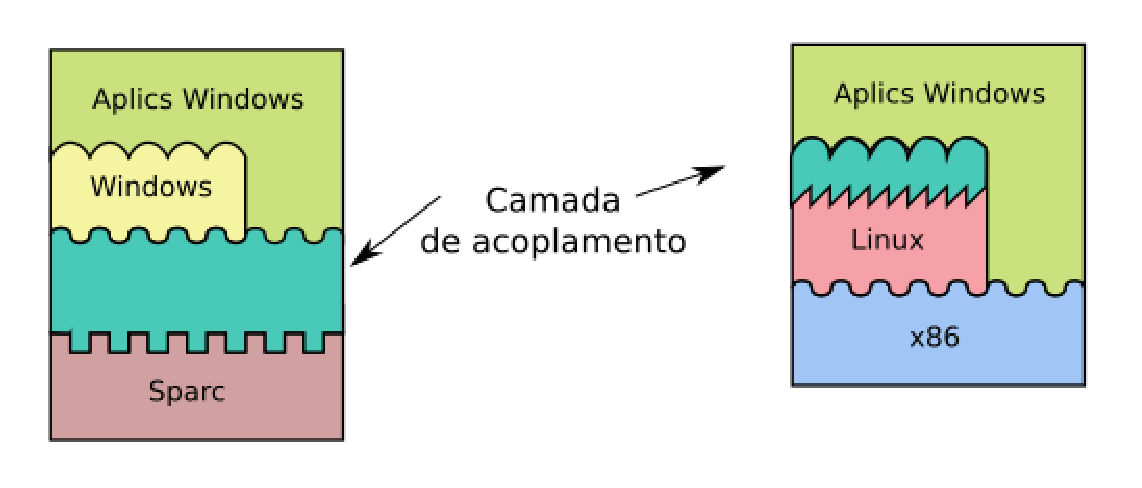
\includegraphics[height=140px]{img/acoplamento_interfaces.eps}
 \caption{Acoplamento entre interfaces distintas}
 \label{fig:acoplamento_interfaces}
\end{figure}
Exemplo de camada de virtualização \ref{fig:acoplamento_interfaces} ....


--------------------------------


Máquinas virtuais podem ser divididas em dois grupos: máquinas virtuais de aplicação e máquinas virtuais de sistema. A primeira faz a
virtualização de uma aplicação, suporta apenas um processo ou aplicação. Um exemplo de máquina virtual de aplicação é a \ac{JVM}. 
A máquina virtual de sistema suporta sistemas operacionais convidados, com suas aplicações executando sobre ele. Um exemplo é o sistema
\textit{VMware} \cite{laureano2008}.
Virtualização de sistema utiliza abstração em sua arquitetura, por exemplo, ela transforma um disco físico em dois discos 
virtuais menores, sendo que esses discos virtuais são arquivos armazenados no disco físico. Sabendo que arquivos são uma abstração
em um disco físico, pode-se dizer que virtualização não é apenas uma camada de abstração do \textit{hardware}, ela faz a reprodução 
do \textit{hardware} \cite{smithenair2005}.
Existem várias formas de implementar a virtualização, por isso elas serão detalhas na Seção \ref{section:tiposvirt}.

\section{Virtualização de aplicação}
\label{section:virtaplicacao}


\section{Virtualização de sistema}
\label{section:virtsistema}


\begin{itemize}
 \item Emulação
 \item Virtualização completa
 \item Paravirtualização
 \item Virtualização baseada em contêineres
\end{itemize}
ver jvm e wine

Um ambiente de virtualização é composto basicamente por três componentes:
\begin{itemize}
 \item Sistema real: também pode ser chamado de hospedeiro, que é o \textit{hardware} onde o sistema de virtualização irá executar;
 \item Camada de virtualização: é conhecida como hipervisor ou também chamado de \ac{VMM}, tem como função criar interfaces virtuais a
 partir de interfaces físicas para a comunicação do sistema real com o sistema virtual;
 \item Sistema virtual: também conhecido como \textit{guest}, ou sistema convidado, que executa sobre o sistema real. Geralmente
 existem vários sistemas virtuais executando simultaneamente sobre o sistema real.
\end{itemize}

\section{Vantagens}
\label{section:vantagensvirt}

Em muitos casos empresas utilizam serviços distribuídos entre servidores físicos, como, por exemplo, servidores de e-mail, hospedagens e 
banco de dados, com isso existe uma ociosidade grande de recursos. Portanto uma das grandes vantagens da virtualização é um melhor 
aproveitamento destes recursos, alocando vários serviços em um único servidor gerando um melhor aproveitamento do \textit{hardware} 
\cite{moreira2006}. Além disso, pode-se ter uma redução de custos com a administração e a manutenção dos servidores. Em um ambiente 
heterogênio pode-se também utilizar virtualização, pois ela permite a instalação de diversos sistemas operacionais em um único servidor.

Uma outra motivação para a utilização de virtualização consiste no custo da energia elétrica. A economia de energia pode ser obtida através 
da implantação de servidores mais robustos para substituir dezenas de servidores comuns. Outros fatores como refrigeração do ambiente e 
espaço físico utilizado também podem ser reduzidos com a implantação de virtualização de servidores, e consequentemente, reduzem os 
custos de energia também.

A virtualização favorece a implementação do conceito um servidor por serviço, que consiste em ter um servidor para cada serviço.
Mas porque não colocar todos serviços em um único servidor? Muitas vezes com uma variedade de serviços é necessário diferentes 
sistemas operacionais, ou os serviços necessitam rodar nas mesmas portas, portanto isto se torna inviável. Outro fator relevante que 
também favorece a implementação de um servidor por serviço é, caso exista uma falha de segurança em apenas um serviço, essa 
vulnerabilidade poderá comprometer todos os outros serviços 
\cite{carissimi2008}.

\section{Funcionamento}
\label{section:funcionamentovirt}

** Anéis de privilégios, compatibilidade, e hypervisor \cite{goncalves2009}.


%Virtualização_ da teoria a soluções.pdf
%virtualizacao mainframes: pag 1 - Alta Disponibilidade em Servidores Virtualizados.pdf
%pag 32 - Rejuvenescimento e migracao de vms - Matheus D'Eça de Melo.pdf
%pag 20 - Implementação de Alta disponibilidade em Máquinas Virtuais utilizando Software Livre.pdf
%ferramentas pag 4 - Main - Virtualização de serviços baseado em contêineres -WandersonReis.pdf

%Virtualizacao da teoria a solucoes:
%No entanto, essa abordagem trouxe como contra-partida a filosofia “um servidor
%por serviço”. Rapidamente, os responsáveis pelas áreas de TI se deram conta do
%problema (e custo) em gerenciar diferentes máquinas físicas, mesmo que tivessem o
%mesmo sistema operacional. Além disso, há problemas relacionados com consumo de
%energia elétrica, refrigeração, espaço físico, segurança física, etc. Nesse contexto, a
%virtualização surge como uma possibilidade de agregar os benefícios da componetização
%de sofware com a redução dos custos de manutenção de hardware e software. Assim, é
%possível manter a idéia de um “um servidor por serviço” sem ter um hardware
%específico.
%Essa abordagem é reforçada pela lei de Zipf [Adamic, 2008] que pode ser
%sintetizada da seguinte forma: a freqüência de um evento é proporcional a x −α , onde x é
%um ranking de comparação de um evento a outro. Alguns estudos [Breslau, Cao, Fan,
%Philips e Shenker, 2008] mostraram que a freqüência de acesso a servidores web e
%outros serviços Internet seguem uma distribuição Zipfian, o que, na prática, se traduz
%pelo fato de que a maioria dos acessos a serviços Internet é para uma minoria deles.
%Portanto, conclui-se que uma minoria de serviços está ativa enquanto a maioria está
%bloqueada a espera de requisições, o que, claramente, representa um desperdício de
%recursos. Para exemplificar, imagine, entre outros, o uso dos servidores de autenticação,
%DHCP, impressão, arquivos, e-mail, web e DNS em sua rede corporativa.

%Rejuvenescimento e migracao de vms:
%Com a arquitetura baseada em serviços, clientes podem utilizar serviços alocados em
%nuvem através dos web browsers. Unindo a computação em nuvem e a arquitetura baseada
%em serviços, aplicativos e demais recursos de TI podem ser oferecidos remotamente, como se
%estivessem localizados localmente. Vale a pena salientar que a arquitetura baseada em serviços
%permite monitorar em tempo real o uso dos recursos disponibilizados, colaborando assim para
%uma gerência mais eficiente a todo o sistema (LINTHICUM, 2009). Além disso, dependendo
%das interfaces definidas, pode-se ampliar consideravelmente o número de potenciais clientes.
%Recursos disponibilizados via navegador web, por exemplo, podem ser acessados tanto por
%computadores de mesa quanto por smartphones ou tablets.
%

%ver failover e failback em cluster?

\chapter{Estudo de caso ? esse titulo ?}
\label{cap:estudodecaso}

Após terem sido compreendidos os conceitos de alta disponibilidade e de virtualização, pode-se iniciar a análise da estrutura atual da empresa.
Essa empresa, que fornece serviços de hospedagens, será o foco desse trabalho, sabendo que ela atualmente possui redundância de refrigeração 
e energia. Assim, essas redundâncias tem como objetivo prover um ambiente físico estável e confiável.

Para ser possível propor uma solução de alta diponibilidade é necessário conhecer o cenário atual da empresa. 
Nas próximas seções serão detalhados: o ambiente físico (Seção \ref{section:estfis}); a estrutura lógica, com a relação de servidores físicos
e virtuais (Seção \ref{section:estlog}); todos os serviços fornecidos pela empresa (Seção \ref{section:serv}); e por fim o levantamento
dos serviços críticos (Seção \ref{section:servcrit}).

\section{Estrutura física}
\label{section:estfis}

A estrutura atual da empresa é composta por quatorze servidores montados em um \textit{rack}. A configuração desses servidores esta listado
na Tabela \ref{tab:servfisicos}.

\begin{table}
\caption {Configuração dos servidores físicos}
\label{tab:servfisicos}
\begin{center}
\begin{tabular}{|l|p{3.8cm}|l|p{3cm}|l|}\hline
Servidor & Processador & Memória & Disco & Marca / modelo\\\hline
bello & Intel Core 2 Duo CPU E6750 2.66GHz & 2GB DDR2 & 5,5TB SATA & \\\hline
brina & 2 x Intel Xeon CPU E5410 2.33GHz & 24GB DDR2 & 6 x 300GB SAS & Dell PowerEdge 2950\\\hline
cacti & 2 x Intel Xeon CPU E5310 1.60GHz & 12GB DDR2 & 2 x 73GB SAS & Dell PowerEdge 2950\\\hline
dati & 2 x Intel Xeon CPU 3.20GHz & 4GB DDR2 & 2 x 146GB SCSI & Dell PowerEdge 1850\\\hline
fulmine & 1 x Intel Xeon CPU E5-2650 2.00GHz & 32GB DDR3 & 6 x 2TB SATA & IBM System x3650 M4\\\hline
monit & Intel Core 2 Quad CPU Q9550 2.83GHz & 4GB DDR2 & 120GB SSD & \\\hline
nino & Intel Core 2 Duo CPU E4500 2.20GHz & 4GB DDR2 & 500GB SATA & \\\hline
piova & 2 x Intel Xeon CPU E5530 2.40GHz & 32GB DDR3 & 4 x 500G SATA & Dell PowerEdge R410\\\hline
raggio & 2 x  Intel Xeon CPU E5630 2.53GHz & 32GB DDR3 & 4 x 300GB SAS & HP ProLiant DL360 G7\\\hline
sfrunhon & Intel Xeon CPU X3330 2.66GHz & 8GB DDR2 & 750GB SATA & \\\hline
tempesta & 2 x Intel Xeon CPU E5-2620 2.00GHz & 32GB DDR3 & 5 x 1TB SATA & Dell PowerEdge R620\\\hline
tuono & 2 x Intel Xeon CPU E5649 2.53GHz & 32GB DDR3 & 6 x 300GB SAS 2 x 146GB SAS & HP ProLiant DL380 G7\\\hline
venti & Intel Xeon CPU E3-1220 3.10GHz & 16GB DDR3 & 2 x 3TB SATA & Dell PowerEdge R210 II\\\hline
vigilante & Intel Pentium Dual CPU E2180 2.00GHz & 4GB DDR2 & 2,5TB SATA & \\\hline
\end{tabular}
\end{center}
\end{table}

-diagrama físico

-graficos cpu memoria disco

\section{Estrutura lógica}
\label{section:estlog}

Atualmente sete servidores são utilizados para virtualização. O primeiro (Figura \ref{fig:servlog_1}), ...

-diagramas máquinas de virtualização

\begin{figure}[servlog_1]
 \centering
 \includegraphics[width=380px]{img/servlog_1.eps}
 \caption{Servidor virtualização.}
 \label{fig:servlog_1}
\end{figure}

\section{Serviços}
\label{section:serv}

A empresa fornece serviços diversos, desde hospedagens de sites até \textit{DNS} recursivo para um provedor de internet.
A Tabela \ref{tab:servporservidor} mostra todos os servidores, incluindo virtuais, e seus respectivos serviços.

\begin{table}
\caption {Serviços por servidor}
\label{tab:servporservidor}

\begin{center}
\begin{tabular}{|l|p{12cm}|}\hline
Servidores & Descrição\\\hline
asp & Servidor web linguagem ASP\\\hline
backup & Servidor de backup equipamentos de rede do provedor\\\hline
bello & Servidor de storage do bacula, para backup dos outros servidores\\\hline
brina & Servidor de virtualização\\\hline
cacti & Servidor de monitoramento da rede do provedor\\\hline
dati & Banco de dados dos servidores de email e cameras\\\hline
dio & Servidor de hospedagem de sites PHP4\\\hline
esibire & Servidor de hospedagem de vídeos\\\hline
fatefurbo & Servidor para gerência da fibra óptica do provedor\\\hline
fiberhome & Servidor para gerência da fibra óptica do provedor\\\hline
fulmine & Servidor de virtualização\\\hline
hotspot & Servidor de gerência de equipamentos da Ubiquiti que fazem hotspot utilizado pelo provedor\\\hline
ledriovardar & Servidor de terminal service do suporte e gerência do provedor\\\hline
masterauth & Servidor de autenticação PPPoE do provedor\\\hline
merak & Servidor de email\\\hline
miatanto & Servidor de streaming Icecast para web rádio\\\hline
mondoperso & Servidor de streaming Icecast de uma rádio ao vivo\\\hline
monete & Servidor de hospedagem de site dedicada do provedor\\\hline
monit & Servidor de monitoramento e gráficos de todos servidores\\\hline
nino & Ambiente de desenvolvimento para setor de programação web\\\hline
ns & Servidor primário de DNS autoritativo\\\hline
ottico & Servidor de terminal service do suporte e gerência de fibra óptica do provedor\\\hline
parla & Servidor de mensagens instantâneas XMPP do provedor\\\hline
passata & Servidor primário de DNS recursivo do provedor\\\hline
passata2 & Servidor secundário de DNS recursivo do provedor\\\hline
piova & Servidor de virtualização\\\hline
pomodoro & Servidor de documentação Sakai do provedor\\\hline
postfix & Servidor de SMTP para envio de email marketing\\\hline
quebei & Servidor de gerência do bacula, para backup dos outros servidores\\\hline
raggio & Servidor de virtualização\\\hline
rauco & Servidor de hospedagens WHM\\\hline
roncon & Servidor de hospedagens WHM\\\hline
ronconradius & Servidor de radius ADSL de terceiros\\\hline
servo & Servidor secundário de DNS autoritativo\\\hline
servo6 & Servidor terciário de DNS autoritativo\\\hline
sfrunhon & Servidor de gráficos para monitoramento de clientes do provedor\\\hline
simplesip & Servidor de telefonia Asterisk do provedor\\\hline
soldi & Servidor de sistemas do provedor e outros ERPs\\\hline
speedauth & Servidor de autenticação PPPoE do provedor\\\hline
tempesta & Servidor de virtualização\\\hline
trapel & Servidor de teste de banda do provedor\\\hline
tuono & Servidor de virtualização\\\hline
venti & Servidor de virtualização\\\hline
vigilante & Servidor de reprodução e armazenamento das câmeras do provedor\\\hline
vinicolag & Servidor de backup de um cliente\\\hline
\end{tabular}
\end{center}
\end{table}


\section{Serviços críticos}
\label{section:servcrit}



\chapter{Proposta de solução}
\label{cap:propostadesolucao}

Neste capítulo será proposto uma solução de implementação de um ambiente de alta disponibilidade para os serviços críticos da empresa, que 
foram selecionados no capítulo anterior. Com isso pretende-se atingir o objetivo deste trabalho.

O primeiro passo desta implementação é fazer uma reorganização das máquinas virtuais entre os servidores atuais, liberando assim o 
\textit{hardware} suficiente para possibilitar a implementação do ambiente de alta disponibilidade. 

Após ter sido feito a reorganização das máquinas virtuais será iniciado a implementação, montando um ambiente com dois servidores e os 
configurando de uma forma que caso houver alguma falha, em um servidor físico ou no seu sistema operacional hospedeiro, as máquinas serão 
tranferidas para o outro servidor físico. 
A configuração deverá ser: 11 \textit{cores} de processamento, 12 GB de memória e 156 GB de disco para cada servidor. Essa configuração foi 
calculada a partir da soma dos recursos atuais das máquinas virtuais que possuem os serviços críticos, que foram apresentadas no capítulo
anterior na Seção \ref{section:servcrit}.

As ferramentas necessárias para essa implementação podem ser divididas em dois tipos: ferramenta de replicação de dados 
(Seção \ref{section:toolrepl}) e ferramenta que faz o monitoramento e a tranferências das máquinas virtuais em caso de falhas 
(Seção \ref{section:toolcluster}).

\section{Ferramentas de replicação de dados}
\label{section:toolrepl}

Replicação de dados pode ser feita de diversas maneiras, pode ser a nível de aplicação ou até mesmo a nível de \textit{hardware}.
Dependendo do objetivo e da aplicação pode-se usar ferramentas como por exemplo o \textit{rsync}, que faz o sincronismo de dados de uma origem
para um destino. Sendo assim, não é possível utilizar essa ferramenta, pois ela não faz a replicação em tempo real, ou seja, se for necessário
utilizar os dados de destino ocorrerá perda de dados. Outra forma de replicação é a de discos com \ac{RAID} por exemplo, essa solução é eficaz
para garantir que o sistema não fique indisponível em caso de falha de discos\footnote{Lembrando que essa solução é utilizada no ambiente atual
para aumentar a disponibilidade dos servidores}, porém não garante a disponibilidade quando algum componente de \textit{hardware} falhar 
\cite{zaminhani2008}.

A solução de replicação ideal para esta implementação é um espelhamento de dados através da redes, assim permitindo a cópia dos dados para uma
máquina remota. Essa solução além de fazer a replicação dos dados, faz a redundância de todo \textit{hardware}.

A ferramenta escolhida para replicação de dados na solução de alta disponibilidade desse trabalho foi o \ac{DRBD}. Essa ferramenta é de código
aberto, e permite a replicação de dados de um dispositivo local em tempo real. 
APROFUNDAR AQUI OU NA IMPLEMENTAÇÂO?

% dispositivo primario e secundario zaminhani2008
% Segundo (ELLENBERG, 2007), a partir da versão 8 do DRBD é possível que,
%dependendo da aplicação, a execução ocorra em todos os nós do cluster
%simultaneamente (Ativo/Ativo). Para tornar isso possível é necessária a
%utilização de um sistema de arquivos exclusivo para cluster, como o OCFS2 6 e o
%GFS 7 por exemplo. Como a abordagem deste trabalho é cluster de alta
%disponibilidade, a utilização do DRBD no modo Ativo/Ativo não será discutida.

\section{Ferramentas de gerenciamento de cluster?}
\label{section:toolcluster}

Para ser possível implementar uma solução de alta disponibilidade é necessário uma ferramenta que monitora os recursos, fazendo a detecção e
recuperação do serviço utilizando mensagens entre os servidores \cite{perkov2011}.

\textit{Pacemaker} é uma ferramenta de detecção e recuperação de falhas a nível de serviço \cite{perkov2011}. 
Continuar ??? \textit{Heartbeat} \cite{zaminhani2008}.


%reorganização de vms
%ferramentas selecionadas, colocar motivo para escolher e citar ferramentas parecidas
%muitos servicos, melhor solucao utilizar 2 servidores para fazer redundancia
%em caso de falha de um servidor fisico...
%ferramentas open source...
%colocar a disponibilidade do nagios do ano passado?


\bibliography{tcc}
\bibliographystyle{abnt}

\end{document}
